% Options here are passed to the article class.
% Most common options: 10pt, 11pt, 12pt
\documentclass[10pt]{datasheet}

% Input encoding and typographical rules for English language
\usepackage[utf8]{inputenc}
\usepackage[english]{babel}
\usepackage[english]{isodate}

% tikz is used to draw images in this example, but you can
% also use \includegraphics{}.
\usepackage{graphicx}
\usepackage{float}
\usepackage{subcaption}

% These define global texts that are used in headers and titles.
\title{DC05: 4-9 Bit Binary Decoder With Top Output}
\author{Basil, Crain}
\tags{decoders, binary}
\date{25 December 2024}
\revision{Revision 1}
\begin{document}
\maketitle

\section{Features}

\begin{itemize}
\item{Can be expanded to up to 9 bits of input.}
\item{Outputs can be taken from the top. (Observe rail state for output)}
\item{11 gt latency and 8 gt throughput.}
\end{itemize}

\section{Applications}

\begin{itemize}
\item{Decoding binary signals for use in encoded systems}
\end{itemize}

\section{General Description}
The DC05 decoder takes 4 bits and outputs a pulse at one of 16 slices corresponding to the code. The device can be expanded to 9 bits of input. The output can be taken from the top of the device.
\vfill\break

\begin{figure}[H]
    \centering
    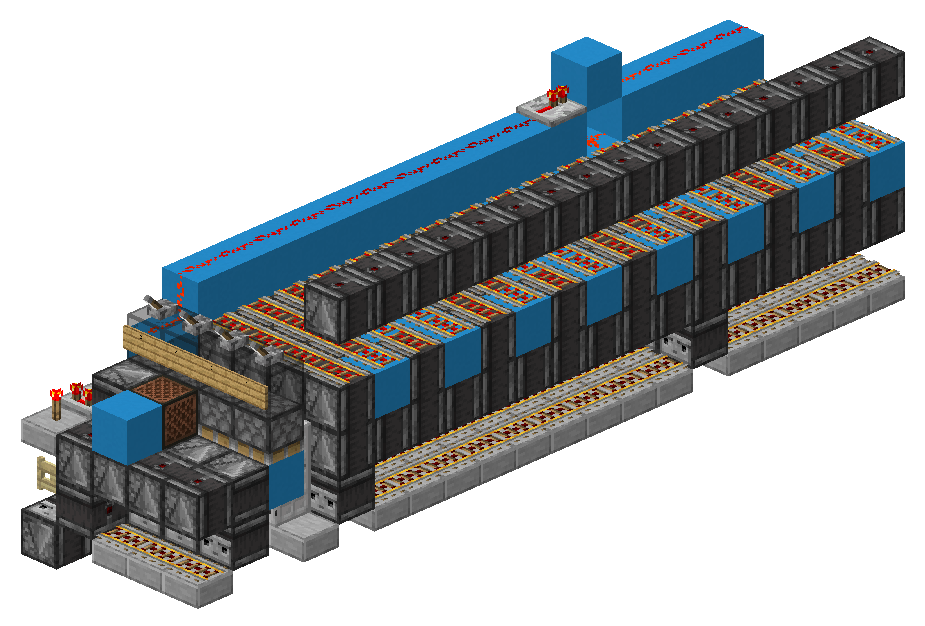
\includegraphics[width=0.48\textwidth]{decoderpic.png}
    \caption{\centering 4 Bit Binary Decoder With Top Output}
\end{figure}

% For wide tables, a single column layout is better. It can be switched
% page-by-page.
\onecolumn

\section{Device Specifications}

\begin{table}[H]
    \caption{Inputs}
    \begin{tabularx}{\textwidth}{l | c | X}
        \thickhline
        \textbf{Name} & \textbf{Range} & \textbf{Description} \\
        \hline
        Bits 1-4 & 0-1 & Binary input \\
        \hline
        Clock & Pulse & Clock signal of device. \\
        \thickhline
\end{tabularx}
\end{table}

\begin{table}[H]
    \caption{Outputs}
    \begin{tabularx}{\textwidth}{l | c | X}
        \thickhline
        \textbf{Name} & \textbf{Range} & \textbf{Description} \\
        \hline
        Mapped signal & Pulse & Outputs to one of 16 slices corresponding to input code. \\
        \thickhline
\end{tabularx}
\end{table}

\begin{table}[H]
    \caption{Device Specifications}
    \begin{tabularx}{\textwidth}{l | c c c | c | X}
        \thickhline
        \textbf{Parameter} & \textbf{Min.} & \textbf{Typ.} & \textbf{Max.} &
        \textbf{Unit} & \textbf{Conditions} \\
        \hline
        Throughput  & 8 & - & - & gt & Normal Usage \\
        \hline
        Latency    & 11 & 11 & 11 & gt & From input to output observer activation. \\
        \hline
        MC Version & 1.13 & 1.19.3 & - & MCV & Latest version at time of writing: 1.21.4\\
        \hline
        Dimensions & & 5 x 6 x 20 & & Blocks & \\
        \thickhline
\end{tabularx}
\end{table}
\section{Testing Data}
\begin{table}[H]
\caption{Executed Tests}
\begin{tabularx}{\textwidth}{l | X}
    \thickhline
    \textbf{Test} & \textbf{Result} \\
    \hline
    Throughput test & Device was able to function with 8gt clocked input. \\
    \thickhline
\end{tabularx}
\end{table}

\section{Download Information}
\begin{table}[H]
    \caption{Download Information}
    \begin{tabularx}{\textwidth}{l | l | l | X}
        \thickhline
        \textbf{Identifier} & \textbf{MC} & \textbf{File} & \textbf{Description} \\
        \hline
        DC05 & 1.19.3 & \href{https://github.com/Soontech-Annals/Archive/blob/8413f90a054b6c415703bae02badeba7541344f6/Archive/decoders/DC05\%204-9\%20Bit\%20Binary\%20Decoder\%20With\%20Top\%20Output/DC05\_4-9\_Bit\_Binary\_Decoder\_With\_Top\_Output.litematic?raw=1}{DC05\_4-9\_Bit\_Binary\_Decoder\_With\_Top\_Output.litematic} & Schematic of device. \\
        \hline
        \thickhline
    \end{tabularx}
\end{table}

\end{document}

